\chapter[La Matrice Densité]{La Matrice Densité}
\label{chap:densite}

\section{Position du problème}
La description physique du phénomène de résonance magnétique nucléaire
peut s'effectuer à (au moins) trois niveaux, faisant appel aux diagrammes énergétiques,
au vecteur d'aimantation macroscopique (le modèle de Bloch) et au formalisme
de la matrice densité.
Le modèle de Bloch, présenté précédemment, donne une image réaliste de 
l'évolution d'un système de noyaux isolés magnétiquement les uns des autres. 
Ce modèle peut être étendu pour y inclure l'action
des couplages scalaires. 
Il a ici semblé utile d'introduire le formalisme de la matrice densité à un 
niveau très élémentaire plutôt que de continuer avec le modèle de Bloch,
afin de faciliter l'étude d'expériences complexes 
faisant appel, par exemple, aux transitions à multiple quanta et
de justifier simplement la structure du programme de phase associé à une séquence 
multi-impulsionnelle. 

S'il est relativement aisé de comprendre comment utiliser
un diagramme énergétique ou une représentation vectorielle,
la caractérisation d'un système physique par une matrice
n'est pas usuellement ressentie comme intuitive.
La matrice densité possède une définition parfaitement rigoureuse dans 
le cadre du formalisme de la mécanique quantique.
Ce dernier n'est pas immédiatement accessible au non-initié,
et aurait même une action fortement répulsive.
Il n'est d'autre part pas évident de justifier 
par la seule compréhension de la RMN
la nécessité de l'assimilation préalable d'un volumineux
corpus de connaissances générales en mécanique quantique.
L'expérience montre qu'il est possible d'utiliser un nombre minimal
de définitions et de règles, sans démonstration, pour parvenir à une
description de la RMN utilisant la matrice densité et
qui soit opérationnelle dans la plus part des situations usuelles.
Le lecteur curieux et séduit par la puissance de cette approche n'en sera que
plus motivé pour aborder l'apprentissage des fondements de la mécanique quantique,
et découvrir l'origine des règles qu'il aura utilisées de prime
abord en toute innocence.
La matrice densité sera donc par la suite un objet dont il sera question
sans qu'une définition formelle ne lui ait été préalablement donnée.
Cette démarche non conventionnelle, surtout au pays de Descartes,
est cependant d'un intérêt certain, même
si elle peut dérouter.

Le concept de matrice densité est utilisé par les physiciens pour décrire le 
comportement d'un ensemble de particules qui ne présentent pas toutes le même état. 
Un système composé d'une particule ou d'un ensemble de particules de 
même état (cette situation est désignée sous l'appellation "cas pur") est 
parfaitement décrit par une fonction d'onde, fonction dont on sait tirer les probabilité de 
mesures de différentes grandeurs observables (position, quantité de mouvement, 
moment cinétique, énergie mécanique totale...) et dont l'évolution dans le temps est 
prévisible grâce à l'équation de Schrödinger.
Un système constitués de $P$ particules de spin 1/2, dont $p_{\al}$ et $p_{\be}$ sont 
dans l'état $m_s = +1/2$ et $m_s = -1/2$ ne peut être correctement 
décrit par une fonction d'onde.
Cette situation (appelée cas impur, ou mélange statistique) est celle
présentée par échantillon en équilibre (au sens thermodynamique du terme) dans un 
champ magnétique, au début de toute expérience de RMN. 
Dans un cas pur, matrice densité et fonction d'onde sont deux représentations 
équivalentes du système considéré. 
Il est possible de déduire de la matrice densité tous les résultats des 
mesures voulues et de déterminer leur évolution au cours du temps. 
Un mélange statistique est la réunion de sous-systèmes purs et 
la matrice densité associée à ce mélange est alors la moyenne 
des matrices densité des sous-systèmes dont il est composé, 
moyenne pondérée par les populations.
La matrice densité dans un cas pur ou dans un cas impur est utilisée de la même manière et 
constitue donc une sorte de généralisation de la fonction d'onde.

Connaissant la matrice densité d'un échantillon dans son état initial et les différents 
événements qui vont survenir (impulsions de radiofréquence entrecoupées de délais 
d'évolution), il sera possible de déterminer la matrice densité à chaque instant de 
l'acquisition du signal de précession libre. 
La grandeur observable, qui est la 
composante horizontale du moment magnétique de l'échantillon, sera déduite de la 
matrice densité.

Une matrice, d'une manière générale, est la représentation d'une transformation (ou opérateur)
linéaire qui transforme un élément d'un espace vectoriel en un autre élément
d'un espace vectoriel (le même ou un autre), ces espaces étant définis sur un même corps
(le corps des nombres complexes, en ce qui concerne ce qui va suivre).
Si le vecteur d'origine appartient à un espace de dimension $m$ et celui
d'arrivée à un espace de dimension $n$,
la matrice qui représente la transformation est un tableau de nombres complexes
possédant $n$ lignes et $m$ colonnes.

Pour situer le degré de complexité des calculs à effectuer, il faut savoir qu'analyser un 
système de $n$ spins couplés nécessite la manipulation de matrices à $2^n$ lignes et $2^n$ 
colonnes! 
De tels calculs sont très largement simplifiés si la matrice densité est 
exprimée comme une somme de matrices, multiples de matrices de base judicieusement 
choisies. 
La taille $n$ du système de spins étant fixée, il y a autant
de matrices de base que d'éléments dans la matrice soit $4^n$. 
Les matrices de base sont désignées sous forme symbolique facile à mémoriser. 
Bien qu'il existe une infinité d'ensembles possibles de matrices de base,
les "produits d'opérateurs cartésiens" seront préférentiellement choisis comme base.
Une base (c'est-à-dire un ensemble de matrices de base) étant choisie, 
des règles de calcul permettent de prévoir l'évolution de la 
matrice densité pendant les évènements qui constituent une séquence d'impulsions.
Chaque événement, impulsion ou délai, est associé à une opération linéaire
qui transforme la matrice densité du système avant l'événement en la matrice densité
après l'événement.
Une telle transformation, qui associe une matrice à une autre matrice, 
est appelée "super--opérateur".

Les règles d'évolution et d'utilisation de la matrice densité seront d'abord
introduites à propos des systèmes à un et deux spins.
D'autres règles permettront de calculer les grandeurs observables
$\aimxs$ et $\aimys$, projections de l'aimantation sur les axes
transversaux du référentiel tournant.
La généralisation de ces règles aux systèmes plus 
complexes procède des mêmes méthodes de calcul. 

\section{Le système à un spin}
\subsection{Les opérateurs cartésiens}
Un système à un spin (pour lequel on peut espérer retrouver les résultats du modèle de 
Bloch) est formé d'un noyau que l'on note $I$.
Les quatre matrices de base qui constituent la base d'opérateurs cartésiens
seront désignées par $E/2$, $I_x$, $I_y$ et $I_z$.
D'une manière générale, la matrice densité du système de spins considéré peut toujours s'écrire
\begin{equation}
\sigma = a \cdot E/2 + b \cdot I_x + c \cdot I_y + d \cdot I_z
\end{equation}
où $a$, $b$, $c$ et $d$ sont des nombres réels.
Les matrices $I_x$, $I_y$ et $I_z$ sont aussi appelées les matrices de Pauli.
La matrice identité $E$ intervient sous forme de E/2 pour des raisons
d'homogénéité des propriétés des matrices de base.
Les quatre matrices de base permettent de définir tout état du système de spins.
L'ensemble de tous les états possible constitue ce qui est appelé l'\emph{espace des états}.

\subsection{État initial}
La matrice densité, notée $\sigma$, d'un ensemble de $P$ noyaux plongé dans un champ magnétique, 
et ayant atteint une situation d'équilibre est :
\begin{equation}
\sigma_0 = P \cdot E/2 + \Delta P \cdot I_z
\end{equation}
où $\Delta P$ est la différence des populations initiales $p_{\al} - p_{\be}$ 
(voir p. \pageref{page:population}). 
La matrice $E$ étant la matrice identité, sa transformation par un opérateur linéaire
donnera toujours la matrice identité.
Sa contribution à $\sigma$ n'évolue pas au cours du temps.
Pour cette raison le terme proportionnel à $E/2$ sera toujours omis 
dans la suite des calculs. 
Ainsi,
\begin{equation}
\sigma_0 = \Delta P \cdot Iz
\end{equation}
Le coefficient multiplicatif $\Delta P$ se retrouvera tout au long du calcul de l'évolution
de la matrice densité du système, par linéarité des transformations qu'elle subit. 
Par souci de clarté, ce facteur sera aussi omis dans les calculs. 
Néanmoins, si on veut comparer différentes techniques du point de vue quantitatif, 
il est nécessaire de se souvenir de l'existence de ce facteur.
L'état initial du système sera donc décrit par :
\begin{equation}
\sigma_0 = I_z
\end{equation}

\subsection{Évènements}
\label{sec:evenements}
L'effet d'une impulsion ou de l'évolution libre du système pendant un délai
est calculé par action d'un super-opérateur sur la matrice densité. 
Par linéarité, si une matrice $\sigma$ est la somme de deux matrices
$I_a$ et $I_b$ ($a$ ou $b$ = $x$, $y$, ou $z$) multipliées par les 
coefficients $a$ et $b$ :
\begin{equation}
\sigma =  a \cdot I_a + b \cdot I_b
\end{equation}
et si $\hat{O}$ est le super-opérateur associé à un événement 
(impulsion ou délai) alors $\sigma'$, transformée de $\sigma$ par $\hat{O}$, 
se déduit des transformées de $I_a$ et $I_b$ par $\hat{O}$ :
\begin{equation}
\sigma' = \hat{O}(\sigma) = a \cdot \hat{O}(I_a) + b \cdot \hat{O}(I_b)
\end{equation}
Il suffit donc de connaître le résultat de la transformation des matrices de base pour 
calculer le résultat de la transformation de toute matrice.

Tout événement est caractérisé par l'\emph{interaction} entre les spins et l'extérieur
ainsi que par sa \emph{durée}.
Une interaction est \emph{caractérisée} par son \emph{intensité} et sa \emph{nature},
supposées constantes pendant toute la durée où elle s'applique. 
Cela sera vrai pour les impulsions et les délais considérés dans le référentiel tournant.
C'est pourquoi les analyses théoriques qui seront conduites par la suite 
se feront dans implicitement dans le référentiel tournant.
La \emph{description} d'une interaction sera effectuée au moyen d'une matrice, 
dont la nature mathématique est identique à celle de la matrice densité du système.
Une interaction est donc décrite par une matrice, elle même associée à un opérateur
appelé opérateur \emph{hamiltonien}.
L'action d'un hamiltonien $H$ (les exemples arrivent bientôt, patience...)
constant pendant un temps $t$ sur la matrice densité 
d'un système se traduit par un super-opérateur $\hat{H}$ qui ne dépend
que du produit $H \cdot t$, et ceci selon une relation mathématique qui
est sans intérêt à ce niveau de l'exposé. 
En résumé :
\begin{equation}
\sigma \flham{H \cdot t} \sigma' = \hat{H}(\sigma)
\end{equation}
On commettra par la suite un abus de langage en parlant de la transformation
de la matrice densité sous l'action de l'opérateur $Ht$, alors qu'il
faudrait parler de l'action du super-opérateur calculé à partir du produit $Ht$.

Les opérateurs associés aux impulsions de radio-fréquence
dépendent de leur phase $\phi$ et de l'amplitude $\buns$ de leur
champ de radiofréquence caractérisée par la pulsation $\omuns$.
Si l'impulsion dure un temps $t$, l'angle $\theta$ de basculement
de l'aimantation est $\theta = \omuns t$.
Nous nous plaçons ici dans l'hypothèse où l'effet d'offset est négligeable
et donc où $|\omzeros| \ll |\omuns|$.
Les impulsions seront alors dites parfaites car l'aimantation
n'évolue que dans un plan strictement vertical du référentiel tournant.

Si la phase d'une impulsion de RF vaut 
0, $\pi/2$, $\pi$ ou $-\pi/2$, l'opérateur correspondant sera noté
$\omuns I_x$, $\omuns I_y$, $-\omuns I_x$ ou $-\omuns I_y$.
Dans leur forme explicite, les opérateurs d'évolution sont en effet 
semblables aux "opérateurs cartésiens" utilisés comme matrices de base. 
En commettant l'abus de langage mentionné ci-dessus, des impulsions de durée $t$
et d'angle de basculement $\theta$ sont donc associées aux opérateurs
$\theta I_x$, $\theta I_y$, $-\theta I_x$ ou $-\theta I_y$,
puisque $\omuns t = \theta$.

Un noyau d'offset $\omzeros$ évoluant librement subit une interaction
$H = \omzeros \cdot I_z$. 
Si cette interaction se prolonge pendant le temps $t$, l'opérateur qui
est associé à l'évolution du système est $\omzeros t I_z = \theta I_z$
où $\theta$ est ici l'angle de précession de l'aimantation dans le
référentiel tournant.

On constate déjà que les noms des matrices de base n'ont pas été choisis
au hasard puisque qu'un opérateur $\theta I_i$ ($i$ = $x$, $y$ ou $z$) 
est associé à une rotation de l'aimantation d'un angle $\theta$ autour de l'axe $Oi$
du référentiel tournant (en écrivant $i$ en majuscule).

\subsection{Transformation des matrices de base}
\label{subsec:transf}
Il faut maintenant savoir comment les matrices de base $I_i$ sont transformées
sous l'action des opérateurs $\theta I_j$ pour prédire toute évolution
de l'aimantation de l'échantillon.
Pour ce faire, il faut préalablement définir le \emph{commutateur} 
$[A,B]$ de deux matrices $A$ et $B$ :
\begin{equation}
[A,B] = A \cdot B - B \cdot A = i.\{A,B\}
\end{equation}
où $A \cdot B$ représente la matrice obtenue par application successive de $B$ et de $A$
et $\{A,B\}$, une notation utile dans le contexte et que
l'auteur désignera par la suite, abusivement certes, comme le
commutateur de $A$ et de $B$, la définition "officielle" (avec des crochets au lieu
d'accolades) de ce terme
introduisant sans nécessité le nombre complexe $i$ dans les calculs.
Le commutateur de $A$ et de $B$ est nul si appliquer d'abord $B$ puis $A$
revient toujours au même qu'appliquer $A$ puis $B$ (d'où le nom de commutateur).

Une matrice de base $I_i$ reste invariante si l'opérateur 
$\theta I_j$ qui lui est appliqué commute avec $I_i$.
Ceci n'est vrai que si $i$ et $j$ sont égaux, c'est-à-dire si $I_i = I_j$.
Dans le cas contraire
\begin{equation}
I_i \flham{\theta I_j} 
\cos\theta \cdot I_i + \sin\theta \cdot \{I_i,I_j\}
\end{equation}

Les commutateurs se déduisent des règles de calcul suivantes :
\begin{equation}
\label{eqn:commutsimple}
\{I_x,I_y\} = I_z \quad \{I_y,I_z\} = I_x \quad \{I_z,I_x\} = I_y
\end{equation}
\begin{equation}
\{I_i,I_j\} = - \{I_j,I_i\}
\end{equation}

\subsection{Mesure des composantes de l'aimantation}
Le vecteur aimantation macroscopique est déterminé à chaque instant par
ses trois composantes $\aimxs$, $\aimys$ et $\aimzs$, elles mêmes
déduites de la matrice densité du système comme les coefficients
de $I_x$, $I_y$, et $I_z$, à un facteur multiplicatif $\gamma\hbar / 2$ près.
Si 
\begin{equation}
\sigma = a \cdot E + b \cdot I_x + c \cdot I_y + d \cdot I_z
\end{equation}
alors
\begin{equation}
\aimxs = b\gamma\hbar/2 \quad 
\aimys = c\gamma\hbar/2 \qetq 
\aimzs = d\gamma\hbar/2
\end{equation}
Dans la pratique le facteur $\gamma\hbar/2$ sera implicite, et donc ne
sera jamais écrit, sauf dans le cadre de considération quantitatives
sur l'intensité des signaux.

\subsection{Action d'une impulsion sur l'état d'équilibre}
L'état initial de l'aimantation de l'échantillon est caractérisé par $\sigma_0 = I_z$.
Si $\sigma_1$ désigne la matrice densité du système après une 
impulsion de phase $\pi/2$ et d'angle $\theta$ (une impulsion $\theta_y$) alors
\begin{equation}
\sigma_1 = \cos\theta \cdot I_z + \sin\theta \cdot \{I_y,I_z\} =  
\cos\theta \cdot I_z + \sin\theta \cdot I_x
\end{equation}

On en déduit qu'à la fin de l'impulsion
\begin{equation}
(\aimxs, \aimys, \aimzs) = (\sin\theta, 0, \cos\theta)
\end{equation}
ce qui correspond, à un facteur multiplicatif $\Delta P \cdot \gamma\hbar/2$ près, 
aux coordonnés du vecteur $\aimvec$ initial après rotation de 
l'angle $\theta$ autour de l'axe $OY$, dans le plan $OXZ$, 
dans le sens trigonométrique (de $OZ$ vers $OX$).
Si $\theta = \pi/2$ alors $\sigma_1 = I_x$ et donc $\aimxs = 1$ et $\aimys = \aimzs = 0$. 
La nullité de $\aimzs$ traduit l'égalité des populations des noyaux pour lesquels 
$m_s = 1/2$ et $m_s = -1/2$.

\subsection{Précession}
Le but est ici de calculer l'aimantation $t$ secondes après une impulsion $\theta_y$.
Sachant que
\begin{equation}
\sigma(0) = \cos\theta \cdot I_z + \sin\theta \cdot I_x
\end{equation}
on déduit par action de l'hamiltonien $\omzeros I_z$ pendant le temps $t$ :
\begin{equation}
\sigma(t) = \cos\theta \cdot I_z + \sin\theta 
(\cos(\omzeros t) \cdot I_x + \sin(\omzeros t) \cdot \{I_z,I_x\}) 
\end{equation}
soit
\begin{equation}
\sigma(t) = \cos\theta \cdot I_z + \sin\theta \cdot \cos(\omzeros t) \cdot I_x\gamma
+ \sin\theta \cdot \sin(\omzeros t) \cdot I_y
\end{equation}
et donc
\begin{equation}
\aimxs = \sin\theta\cos(\omzeros t) \quad 
\aimys = \sin\theta\sin(\omzeros t) \quad 
\aimzs = \cos\theta
\end{equation}

Le vecteur $\aimvec$ évolue en conservant un angle $\theta$ avec la direction du champ $\bzerovec$,
sa composante perpendiculaire à $\bzerovec$ effectue un mouvement circulaire de pulsation $\omzeros$
dans le référentiel tournant, comme prévu.

L'analyse théorique détaillée et rigoureuse des phénomènes de relaxation,
telle qu'elle est présentée dans les ouvrages de référence,
retrace l'évolution de la matrice densité du système étudié sous l'influence
de perturbations aléatoires, et est totalement hors propos ici.
Nous nous limiterons ici à introduire la relaxation par l'approche phénoménologique
des équations de Bloch, comme au chapitre précédent.

Le signal complexe $s(t)$ mesuré dans le référentiel tournant par détection en
quadrature du signal recueilli par les bobines de la sonde sera
\begin{equation}
s(t) = K \cdot \sin\theta \cdot \exp(i \omzeros t) \cdot \exp(-t/T_2^*) \cdot \exp(i\phi)
\end{equation}
où $T_2^*$ est le temps de relaxation transversal apparent de l'aimantation et
$\phi$ un déphasage introduit par l'ensemble des circuit électroniques de
traitement du signal.
Après échantillonnage, numérisation, transformation de Fourier de $s(t)$ et correction de phase, 
le spectre $S(\Omega)$ est obtenu :
\begin{equation}
S(\Oms) = K \cdot \left[ A(\omzeros) + i \cdot D(\omzeros) \right]
\end{equation}
où le coefficient de proportionnalité $K$ contient le produit de 
$\Delta P$, de $\gamma\hbar$ (pour le moment magnétique individuel des noyaux), de
$\gamma\bzeros$ (introduit dans le calcul de la force électromotrice induite),
d'un facteur géométrique qui traduit la distance entre les bobines et l'échantillon,
ainsi que du facteur de surtension électrique $Q$ du circuit oscillant dans lequel
les bobines sont insérées.
Tous calculs faits
\begin{equation}
K \propto P \frac{\gamma^3 \bzeros^2}{T}
\end{equation}

\subsection{A propos de la méthode}
La démarche suivie ici se résume dans les étapes suivantes :
\begin{itemize}
\item Écrire l'expression de l'état (la matrice densité) initiale du système
\item Pour chaque événement, écrire l'opérateur d'évolution correspondant et calculer
son action sur l'état du système
\item Calculez l'état à chaque instant $t$ de la détection du signal, sachant que pendant cette
période le système est soumis à son évolution libre (sauf découplage)
\item Déterminez le signal $s(t)$ par le calcul de
l'aimantation transversale du système à chaque instant $t$
\item Calculez la transformée de Fourier du signal pour déterminer le spectre recherché
\end{itemize}

La méthode décrite ici est très générale et s'inspire de la mécanique rationnelle
où l'écriture de l'hamiltonien (classique, par opposition à quantique) d'un système
conditionne l'écriture des équations différentielle du mouvement.
Leur résolution permet de prévoir l'évolution des positions et des vitesses
du système étudié.

Par ailleurs, on constate la parfaite équivalence entre le modèle vectoriel
de l'aimantation développé au chapitre \ref{chap:bloch} et 
l'approche utilisant la matrice densité.
Cela a pour origine l'équivalence qu'il y a entre les composantes de l'aimantation
et les coefficients multiplicatifs des opérateurs cartésiens $I_x$, $I_y$ et $I_z$.
De plus, les opérations de rotation dans l'espace physique où évolue le vecteur
aimantation ont leurs stricts analogues avec les opérateurs d'évolution, en termes
d'angle et de direction de rotation.
La situation va changer sensiblement pour des systèmes de spins couplés.

\section{Système de deux spins faiblement couplés}

Les matrices de base nécessaires au traitement d'un problème à 2 noyaux sont au 
nombre de $4^2$ soit 16.
D'un point de vue quantique, l'espace des fonctions d'ondes pour un système
de 2 particules est défini comme un \emph{espace produit direct}.
Cette notion de produit direct possède bien entendu une définition mathématique précise.
A ce niveau, il suffit de considérer que c'est une manière d'associer
deux espaces utilisés pour décrire individuellement l'état de deux particules
indépendantes pour former l'espace des états des deux particules prises dans leur ensemble.
Une base de l'espace produit pourrait être constituée en calculant l'ensemble des 
produits directs des éléments des bases associées à chaque des particules.
La base des opérateurs cartésiens d'un noyau $I$ est $\{E_I, I_x, I_y, I_z\}$ et celle
d'un noyau $S$ est $\{E_S, S_x, S_y, S_z\}$.
Par exemple, le produit direct des matrices $I_x$ et $S_y$ devrait s'écrire $I_x \otimes S_y$.
Par commodité, et parce qu'il n'y aura jamais ambiguïté avec le produit interne (celui
qui correspond à l'application successive d'opérateurs à l'intérieur d'un même
espace d'états d'une particule), cette notation deviendra $I_xS_y$.

De la même manière que c'est $E/2$ et non pas $E$ qui est considéré comme matrice de
base lorsqu'il n'y a qu'une particule, des facteurs multiplicatifs
sont nécessaires pour définir la base des \emph{produits d'opérateurs cartésien}
d'un système de deux (et plus de deux) noyaux.
On définit ainsi :
\begin{itemize}
\item $E_IE_S/2 =  E/2$
\item $E_IS_x$, $E_IS_y$, $E_IS_z$ notées $S_x$, $S_y$, $S_z$
\item $I_xE_S$, $I_yE_S$, $I_zE_S$ notées $I_x$, $I_y$, $I_z$
\item $2I_zS_z$, $2I_zS_x$, $2I_zS_y$, $2I_xS_z$, $2I_yS_z$
\item $2I_xS_x$, $2I_xS_y$, $2I_yS_x$, $2I_yS_y$
\end{itemize}

Le facteur 2 présent dans les neuf dernières matrices de base se justifie pour conserver à 
leur ensemble certaines propriétés. 
Ce facteur restera inséparable du reste du symbole des matrices, 
il ne sera jamais inclus dans d'autres facteurs multiplicatifs : $a \cdot 2I_zS_z$
ne sera jamais écrit $2a \cdot I_zS_z$.

\subsection{Etat initial}
L'état initial d'un système de deux noyaux est décrit par la matrice densité
\begin{equation}
\sigma_0 = \Delta P(I)/2 \cdot I_z + \Delta P(S)/2 \cdot S_z
\end{equation}
en omettant le terme constant $1/2 \cdot E/2$. 
Si le système est homonucléaire les différences de population des noyaux $I$ et $S$
sont identiques et dans ce cas $\sigma_0$ est noté $I_z + S_z$. 
Dans le cas contraire, $\Delta P(I)$ et $\Delta P(S)$ sont proportionnels aux rapports 
gyromagnétiques $\gi$ et $\gs$. 
En notant $a = \gs/\gi$, $\sigma_0$ s'écrit $I_z + a \cdot S_z$.

\subsection{Impulsions de radio-fréquence}
Les impulsions de radiofréquence, telles qu'elles ont été présentées au chapitre précédent,
sont non sélectives dans le cas homonucléaire, ou sélectives dans 
le cas hétéronucleaire.
Autrement dit, une impulsion d'angle $\pi/2$ d'une durée de 10 $\mu$s aura le même
effet sur les noyaux $^1$H d'une molécule mais sera incapable d'agir
sur un noyau de $^{13}$C, et vice-versa.
Dans le cas homonucléaire, l'opérateur associé à une impulsion d'angle 
$\theta$ et de phase nulle est $\theta \cdot I_x + \theta \cdot S_x$. 
Pour connaître le résultat provoqué par l'action du super-opérateur associé à une
somme de deux opérateurs, il suffit d'appliquer successivement les deux 
deux super-opérateurs correspondants, dans n'importe quel ordre,
\emph{sous réserve que les opérateurs commutent}, ce qui sera toujours le cas ici.
Dans le cas hétéronucléaire, une impulsion appliquée au voisinage de la fréquence 
d'un des deux noyaux sera associée à l'opérateur défini pour les systèmes à un spin : 
$\theta \cdot I_x$ ou $\theta \cdot S_x$ pour une impulsion sur I 
ou sur S, de phase nulle et d'angle $\theta$.
La règle qui associe phase de l'impulsion et opérateur d'impulsion reste inchangée
(paragraphe \ref{sec:evenements}).
Dans le cas homonucléaire les impulsions exercées
sur les noyaux $I$ et $S$ ont nécessairement la même phase.

\subsection{Évolution libre}
L'évolution libre du système dans le référentiel tournant 
fait intervenir $\omsi$ et $\omss$, écarts entre les pulsations de 
résonance de $I$ et de $S$ et les pulsations des impulsions appliquées aux noyaux $I$ et $S$. 
Le couplage est caractérisé par la constante de couplage $J$. 
L'opérateur d'évolution libre s'écrit alors :
\begin{equation}
\label{eqn:hcouplefaible}
H_{\mbox{\footnotesize evo}} = \omsi \cdot I_z + \omss \cdot S_z + \pi J \cdot 2I_zS_z
\end{equation}
Les trois termes de cet opérateur commutent entre eux (voir ci-après) et peuvent donc
être appliqués dans n'importe quel ordre.
 
\subsection{Relations de commutation}
Les relations de commutation utiles à ce niveau concernent $I_x$, $I_y$, $S_x$, $S_y$ pour les 
opérateurs d'impulsion et $I_z$, $S_z$, $2I_zS_z$ pour les opérateurs d'évolution libre. 
Les règles suivantes indiquent les paires de matrices de base qui commutent (commutateur nul) et 
leur commutateur dans le cas contraire. Les règles de commutation \ref{eqn:commutsimple}
de $I_x$, $I_y$ et $I_z$ restent valables et s'appliquent identiquement
à $S_x$, $S_y$ et $S_z$.

\begin{enumerate}
\item Tout opérateur commute avec lui-même
\item $\{I_i,S_j\} = 0$ pour tout $i$ et tout $j$ égal à $x$, $y$ ou $z$
\item $\{I_i,2I_iS_j\} = \{S_i,2I_jS_i)\} = 0$ pour tout $i$ et tout $j$ égal à $x$, $y$ ou $z$
\item $\{2I_zS_z,2I_iS_j\} = 0$ pour tout $i$ et tout $j$ égal à $x$ ou $y$
\item $\{2I_zS_z,2I_zS_i\} = \{S_z,S_i\}$ pour tout $i$ égal à $x$, $y$ ou $z$
\item $\{2I_zS_z,2I_iS_z\} = \{I_z,I_i\}$ pour tout $i$ égal à $x$, $y$ ou $z$
\item $\{I_i,2I_jS_k) = 2\{I_i,I_j\}S_k$ pour tout $i$, $j$ ou $k$ égal à $x$, $y$ ou $z$
\item $\{S_i,2I_jS_k) = 2I_j\{S_i,S_k\}$ pour tout $i$, $j$ ou $k$ égal à $x$, $y$ ou $z$
\end{enumerate}

Ainsi par exemple :
\begin{enumerate}
\item $\{I_z,I_z\} = 0$
\item $\{I_x,S_z\} = 0$
\item $\{I_z,2I_zS_x\} = \{S_x,2I_yS_x\} = 0$
\item $\{2I_zS_z,2I_yS_x\} = 0$
\item $\{2I_zS_z,2I_zS_y\} = \{S_z,S_y\} = -S_x$
\item $\{2I_zS_z,2I_xS_z\} = \{I_z,I_x\} = I_y$
\item $\{I_x,2I_yS_z\} = 2\{I_x,I_y\}S_z = 2I_zS_z$
\item $\{S_x,2I_zS_z\} = 2I_z\{S_x,S_z\} = -2I_zS_y$
\end{enumerate}

\subsection{Calcul du signal}
Pour un système homonucléaire, $s_x(t)$ (resp. $s_y(t)$) 
se calcule comme la somme des 
coefficients multiplicatifs présents devant $I_x$ et $S_x$ 
(resp. $I_y$ et $S_y$). 
Pour un système hétéronucléaire, la détection du signal n'est réalisée 
que soit aux fréquences de $I$, 
soit à celles de $S$. 
Si on choisit de détecter les signaux des noyaux $I$, $s_x(t)$ et $s_y(t)$ 
se déduisent des coefficients de $I_x$ et $I_y$.

\subsection{Exemple}
Considérons un système $IS$ homonucléaire en équilibre, soumis à une impulsion d'angle 
$\pi/2$ et de phase $\pi/2$.
\begin{equation}
\sigma_0 = I_z + S_z
\end{equation}

$I$ et $S$ jouent ici des rôles complètement symétriques, le résultat de l'évolution de $S_z$ se 
déduit de celle $I_z$ en permutant $I$ et $S$.

L'opérateur d'impulsion est $\pi/2 \cdot (I_y + S_y)$. 
La matrice $I_z$ n'évolue pas sous l'action de $\pi/2 \cdot S_y$ 
car $I_z$ et $S_y$ commutent. 
\begin{eqnarray}
\sigma_1 & = & \cos(\pi/2) \cdot I_z + 
\sin(\pi/2) \cdot \{I_y,I_z\} + \mbox{sym}(I,S) \\
         & = & I_x + \mbox{sym}(I,S) \\
	 & = & I_x + S_x
\end{eqnarray}
La notation sym$(I,S)$ signifiant le résultat de la permutation de 
$I$ et de $S$ dans l'expression qui précède.

Après un temps $t$ d'évolution libre, 
la matrice $\sigma(t)$ se déduit par action successive 
des opérateurs $\omsi t \cdot I_z$, $\omss t \cdot S_z$ 
et $\pi J t \cdot 2I_zS_z$.

Puisque $I_x$ et $S_z$ commutent, l'opérateur 
$\omss t \cdot S_z$ est sans action sur $I_x$.
Ainsi,
\begin{eqnarray}
I_x & \flham{\omsi t \cdot I_z} &
\cos(\omsi t) \cdot I_x + 
\sin(\omsi t) \cdot \{I_z, I_x\} = 
\cos(\omsi t) \cdot I_x + \sin(\omsi t) \cdot I_y \nonumber\\
& \flham{\pi J t \cdot 2I_zS_z} & 
\cos(\omsi t) 
(\cos(\pi J t) \cdot I_x + \sin(\pi J t) \cdot \{2I_zS_z, I_x\}) \nonumber\\
& & +\sin(\omsi t) 
(\cos(\pi J t) \cdot I_y + \sin(\pi J t) \cdot \{2I_zS_z, I_y\})
\end{eqnarray}
Sachant que $\{2I_zS_z, I_x\} = 2I_yS_z$ et que $\{2I_zS_z, I_y\} = -2I_xS_z$
et en développant tous les termes :
\begin{eqnarray}
\sigma(t) & = & \cos(\omsi t) \cos(\pi J t) \cdot I_x
+ \sin(\omsi t) \cos(\pi J t) \cdot I_y \nonumber\\
&  & + \cos(\omsi t) \sin(\pi J t) \cdot 2I_yS_z
- \sin(\omsi t) \sin(\pi J t) \cdot 2I_xS_z \nonumber\\
\label{eqn:evolix-is}&  & + \mbox{sym}(I,S)
\end{eqnarray}

Les termes qui contiennent les opérateurs $I_x$, $I_y$, $S_x$ et $S_y$
sont les seuls à contribuer à la mesure du signal $s(t)$
à l'instant $t$ :
\begin{eqnarray}
s(t) & = & \cos(\pi J t) 
(\cos(\omsi t) + i.\sin(\omsi t)) + \mbox{sym}(I,S) \\
& = & \cos(\pi J t) \exp(i \omsi t) + \mbox{sym}(I,S)
\end{eqnarray}

La première des deux identités
\begin{eqnarray}
\cos(x) & = & \frac{\exp(ix) + \exp(-ix)}{2} \\
\sin(x) & = & \frac{\exp(ix) - \exp(-ix)}{2i}
\end{eqnarray}
permet d'exprimer le signal complexe de façon à 
en faciliter la transformée de Fourier :
\begin{eqnarray}
s(t) & = & \exp(i(\omsi + \pi J)t) / 2 + \exp(i(\omsi - \pi J)t) / 2 
\nonumber\\
&   & + \exp(i(\omss + \pi J)t) / 2 + \exp(i(\omss - \pi J)t) / 2 
\end{eqnarray}
les facteurs liés à la relaxation transversale apparente étant omis
mais implicitement présents.
La transformation de Fourier de cette expression fait apparaître
quatre raies spectrales aux pulsations $\omsi - \pi J$,
$\omsi + \pi J$, $\omss - \pi J$ et $\omss + \pi J$,
c'est-à-dire aux fréquences 
\begin{eqnarray}
\nu_1 & = & \nu_I - J/2 \\ 
\nu_2 & = & \nu_I + J/2 \\
\nu_3 & = & \nu_S - J/2 \\
\nu_4 & = & \nu_S + J/2
\end{eqnarray}
La constante de couplage $J$ est mesurable sur le spectre
en remarquant que :
\begin{equation}
J = \nu_2 - \nu_1 = \nu_4 - \nu_3
\end{equation}

On reconnaît ici le spectre caractéristique d'un système AX (figure \ref{fig:ixy-is})
Le facteur 1/2 traduit que les deux 
composantes de chaque doublet ont une intensité deux fois plus 
faible que les pics produits par les 
noyaux I et S s'ils étaient isolés.

Si, au lieu de déterminer le résultat de l'évolution libre de $I_x$,
c'est celle de $I_y$ qui avait été considérée, le résultat aurait été identique,
à ceci près que les raies du doublet auraient été des raies lorentziennes en dispersion.

\begin{figure}[hbt]
\begin{center}
$a$\hspace{1.5in}\hspace{1cm}$b$\hspace{1.5in}$\mbox{ }$\\
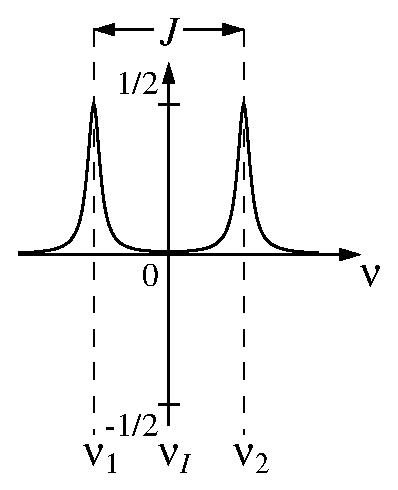
\epsfig{file=ix-is.eps,width=1.5in} \hspace{1cm}
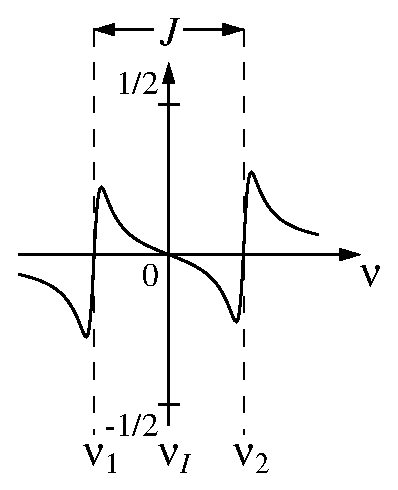
\epsfig{file=iy-is.eps,width=1.5in} \\[1cm]
\end{center}
\caption[Doublets produits par un système $IS$]{
\label{fig:ixy-is}
(a) doublet en absorption issu de $I_x$,
(b) doublet en dispersion issu de $I_y$}
\end{figure}

Si les noyaux $I$ et $S$ ne sont pas de même nature, 
l'impulsion qui excite par exemple l'aimantation du noyau $I$
est sans action sur le noyau $S$.
La détection aux fréquences de $I$ fait 
apparaître un doublet aux fréquences $\nu_1 = \nu_I + J/2$ et
$\nu_2 = \nu_I - J/2$ et rien n'est détectable dans la gamme des
fréquences de résonance de $S$.
Il suffit pour s'en convaincre d'éliminer du calcul
qui précède les termes qui disparaissent si l'opérateur
lié à l'impulsion est seulement $\pi/2 \cdot I_y $
au lieu de $\pi/2 \cdot (I_y + S_y)$.

Dans l'expérience impulsion-détection qui vient d'être décrite 
le signal dû au
noyau $I$ provient de l'évolution de $I_z$ et de $I_z$ uniquement. 
Ce sera toujours le cas pour ce type d'expérience quel que 
soit le nombre de noyaux couplés à $I$.

\section{Systèmes à trois spins (ou plus), faiblement couplés}

\subsection{Méthode}
Conformément à ce qui précède, il faut $4^3 =$ 64 matrices de base pour
décrire l'état d'un système $ISL$ où les trois noyaux sont couplés :

\begin{itemize}
\item La matrice identité $E$, sous forme $E/2$
\item $I_i$, $S_i$ et $L_i$ où $i$ vaut $x$, $y$ ou $z$ (9 matrices)
\item $2I_iS_j$, $2I_iL_j$, $2S_iL_j$ où $i$ et $j$ 
valent $x$, $y$ ou $z$ (27 matrices)
\item $4I_iS_jL_k$ où $i$,$j$ et $k$ valent $x$, $y$ ou $z$ (27 matrices)
\end{itemize}
L'état d'équilibre d'un tel système est défini par la matrice densité 
\begin{equation}
\sigma_0 = \Delta P(I)/4 \cdot I_z + \Delta P(S)/4 \cdot S_z + 
\Delta P(L)/4 \cdot L_z
\end{equation}
Cette écriture se simplifie si le système est homonucléaire : 
\begin{equation}
\sigma_0 = I_z + S_z + L_z
\end{equation}
et si l'aspect quantitatif des calculs qui suivent n'est pas
essentiel.

Les opérateurs associés aux impulsions d'angle $\theta$ sont 
$\epsilon \theta \cdot I_i$, où $i$ vaut $x$ 
ou $y$ et $\epsilon$ 1 ou $-1$ selon la phase de l'impulsion. 
Si plusieurs noyaux sont concernés par une 
impulsion (2 ou 3 noyaux sont de même nature), 
les opérateurs associés sont appliqués successivement.

Les opérateurs d'évolution associés aux déplacements chimiques de 
$I$, $S$ et $L$ sont $\omsi t \cdot I_z$, 
$\omss t \cdot S_z$ et $\omsl t \cdot L_z$. 
Les opérateurs associés au couplage scalaire sont les même que pour 
les systèmes à deux noyaux. 
Il n'existe pas de "super-couplage" qui ferait intervenir 
simultanément les trois noyaux et donc des opérateurs de type 
$4I_zS_zL_z$.

Les règles de commutation ont la même structure que celles utilisées 
pour les systèmes à deux spins. 
Ainsi, par exemple :
\begin{itemize}
\item $\{2I_zS_z,2S_xL_x\} = 4I_z\{S_z,S_x\}L_x = 4I_zS_yL_x$
\item $\{2I_zS_z,2S_zL_y\} = 4I_z\{S_z,S_z\}L_y = 0$
\item $\{2I_zS_z,4I_xS_yL_x\} = 2\{2I_zS_z,2I_xS_y\}L_x = 0$
\item $\{2I_zS_z,4I_xS_zL_y) = 2\{2I_zS_z,2I_xS_z\}L_y = 2I_yL_y$
\end{itemize}

Si par exemple, les noyaux $I$ et $L$ sont de même nature 
et que le signal est détecté à leur 
fréquence, $\aimxs$ (respectivement $\aimys$) est la somme des coefficients
multiplicatifs de $I_x$ et $L_x$  (respectivement $I_y$ et $L_y$).

\subsection{Exemple}
\label{sec:isl}
Considérons un noyau $I$ d'un certain type, couplé à des 
noyaux $S$ et $L$ d'un autre type.
Ce système est caractérisé par trois constantes de 
couplage : $J_{IS}$, $J_{IL}$ et $J_{SL}$. 
A titre d'exemple, considérons l'évolution du noyau $I$, 
soumis d'abord à une impulsion $\pi/2_y$, puis à 
une évolution libre pendant laquelle le signal est enregistré.

Initialement on considérera que $\sigma_0 = I_z$. 
Comme cela se vérifie aisément, seul ce terme fournira un signal détectable à 
la fréquence du noyau $I$.
L'opérateur associé à l'impulsion est comme précédemment $\pi/2 \cdot I_y$.
L'état $\sigma_0$ devient $\sigma_1 = I_x$.
L'opérateur d'évolution comprend 6 termes : $\omss t \cdot S_z$,
$\omsl t \cdot L_z$, $\pi J_{SL} t \cdot 2S_zL_z$, $\omsi t \cdot I_z$, 
$\pi J_{IS} t \cdot 2I_zS_z$ et $\pi J_{IL} t \cdot 2I_zL_z$.
Les trois premiers termes commutent avec $I_x$, il suffit donc d'appliquer les trois 
derniers à $I_x$ pour calculer $\sigma(t)$. 

Les calculs sont menés de façon commode lorsqu'ils 
sont présentés sous forme graphique, comme sur la figure \ref{fig:isl}. 
L'action d'un opérateur $\theta \cdot A$ qui commute avec une 
matrice de base $B$ se traduit par une double flèche verticale.
Dans le cas contraire une 
flèche vers la gauche mène à la copie de la matrice de base $B$ considérée 
et une flèche vers la droite mène au commutateur de l'opérateur et de la matrice de base,
c'est-à-dire à $\{A,B\}$. 
Une flèche à gauche est associée au facteur multiplicatif $\cos(\theta)$, 
une flèche à droite est associée à $\sin(\theta)$. 
Dans le cas où $\theta$ vaut $\pm \pi/2$ la flèche vers la droite est 
associée au coefficient nul ($\sin(\pm\pi/2)$), 
on ne trace alors qu'une simple flèche verticale.
Sur la droite du schéma sont indiqués les opérateurs qui interviennent
à chaque étape du calcul.

\begin{figure}[hbt]
\setlength{\unitlength}{0.9mm}
\begin{center}
\begin{picture}(160,80)
 
 \put(70,80){\makebox(0,0)[t]{$\boldsymbol{\sigma_0 = I_z}$}}
 
 \thicklines
 \put(70,76){\vector(0,-1){10}}
 \thinlines
  \put(160,70){\makebox(0,0)[rb]{$\pi/2 \cdot I_y$}}
 \put(70,65){\makebox(0,0)[t]{$\boldsymbol{\sigma_1 = I_x}$}}
 
 \thicklines
 \put(69.8,61){\vector(0,-1){10}} \put(70.2,61){\vector(0,-1){10}}
 \thinlines
  \put(160,55){\makebox(0,0)[rb]
   {$\omss t \cdot S_z + \omsl t \cdot L_z + \pi J_{SL} t \cdot 2S_zL_z$}}
 \put(70,50){\makebox(0,0)[t]{$\boldsymbol{I_x}$}}
 
 \thicklines
 \put(70,46){\vector(-4,-1){40}}
 \thinlines
 \put(70,46){\vector(4,-1){40}}
 \put(30,35){\makebox(0,0)[t]{$\boldsymbol{I_x}$}}
  \put(160,40){\makebox(0,0)[rb]{$\pi J_{IS} t \cdot 2I_zS_z$}}
 \put(110,35){\makebox(0,0)[t]{$2I_yS_z$}}
 
 \thicklines
 \put(30,31){\vector(-2,-1){20}}
 \thinlines
 \put(30,31){\vector(2,-1){20}}
 \put(110,31){\vector(-2,-1){20}}
 \put(110,31){\vector(2,-1){20}}
 \put(10,20){\makebox(0,0)[t]{$\boldsymbol{I_x}$}}
 \put(50,20){\makebox(0,0)[t]{$2I_yL_z$}}
 \put(90,20){\makebox(0,0)[t]{$2I_yS_z$}}
  \put(160,25){\makebox(0,0)[rb]{$\pi J_{IL} t \cdot 2I_zL_z$}}
 \put(130,20){\makebox(0,0)[t]{$-4I_xS_zL_z$}}
 
 \thicklines
 \put(10,16){\vector(-1,-1){10}}
 \put(10,16){\vector(1,-1){10}}
 \thinlines
 \put(50,16){\vector(-1,-1){10}}
 \put(50,16){\vector(1,-1){10}}
 \put(90,16){\vector(-1,-1){10}}
 \put(90,16){\vector(1,-1){10}}
 \put(130,16){\vector(-1,-1){10}}
 \put(130,16){\vector(1,-1){10}}

 \put(0,5){\makebox(0,0)[t]{$\boldsymbol{I_x}$}}
 \put(20,5){\makebox(0,0)[t]{$\boldsymbol{I_y}$}}
 \put(40,5){\makebox(0,0)[t]{$2I_yL_z$}}
 \put(60,5){\makebox(0,0)[t]{$-2I_xL_z$}}
 \put(80,5){\makebox(0,0)[t]{$2I_yS_z$}}
 \put(100,5){\makebox(0,0)[t]{$-2I_xS_z$}}
 \put(120,5){\makebox(0,0)[t]{$-4I_xS_zL_z$}}
  \put(160,10){\makebox(0,0)[rb]{$\omsi t \cdot I_z$}}
 \put(140,5){\makebox(0,0)[t]{$4I_yS_zL_z$}}

\end{picture}
\end{center}
 \caption[Évolution de $2I_x$, système $ISL$]{\label{fig:isl}
 Excitation et évolution libre de l'aimantation d'un noyau $I$
 couplé à deux noyaux $S$ et $L$.}
\end{figure}

Les parties du graphe en gras correspondent uniquement
à la partie utile.
Comme il est facile de s'en rendre compte, les termes de la
dernière ligne qui ne sont pas en gras ne contribuent pas
au signal.
Avec un peu d'habitude il est possible de savoir,
sans faire d'erreur, quelles branches de l'arbre n'ont
aucune chance d'aboutir à de l'aimantation mesurable.
Pour connaître $s_x(t)$ et $s_y(t)$ il suffit de partir de
la racine de l'arbre (située en haut !) et de faire le
produit des facteurs $\sin()$ et $\cos()$ qui aboutissent à
$I_x$ et $I_y$.

Ainsi,
\begin{eqnarray}
s_x(t) & = & \cos( \pi J_{IS} t) \cos(\pi J_{IL} t) \cos(\omsi t) \\
s_y(t) & = & \cos( \pi J_{IS} t) \cos(\pi J_{IL} t) \sin(\omsi t)
\end{eqnarray}

Le signal complexe $s(t)$ vaut donc
\begin{equation}
s(t) = \cos( \pi J_{IS} t) \cos(\pi J_{IL} t) \exp(i \omsi t)
\end{equation}

En transformant les cosinus en exponentielles complexes :
\begin{equation}
s(t) = \frac{1}{4}\exp(i \omsi t)
(\exp(i \pi J_{IS} t) + \exp(-i \pi J_{IS} t))
(\exp(i \pi J_{IL} t) + \exp(-i \pi J_{IL} t))
\end{equation}
dont le développement fournit une somme de 4 termes :
\begin{eqnarray}
s(t) & = & \frac{1}{4} \exp(i (\omsi + \pi J_{IS} + \pi J_{IL}) t) \\
& & + \frac{1}{4} \exp(i (\omsi + \pi J_{IS} - \pi J_{IL}) t) \\
& & + \frac{1}{4} \exp(i (\omsi - \pi J_{IS} + \pi J_{IL}) t) \\
& & + \frac{1}{4} \exp(i (\omsi - \pi J_{IS} - \pi J_{IL}) t)
\end{eqnarray}

La transformée de Fourier de ce signal comporte quatre raies aux fréquences :
\begin{eqnarray}
\nu_1 & = & \nu_I - J_{IS}/2 - J_{IL}/2 \\
\nu_2 & = & \nu_I - J_{IS}/2 + J_{IL}/2 \\
\nu_3 & = & \nu_I + J_{IS}/2 - J_{IL}/2 \\
\nu_4 & = & \nu_I + J_{IS}/2 + J_{IL}/2
\end{eqnarray}

Un tel ensemble de raies constitue un doublet de doublets, dont on peut
extraire les valeurs des constantes de couplage :
\begin{eqnarray}
J_{IS} & = & \nu_3 - \nu_1 = \nu_4 - \nu_2 \\
J_{IL} & = & \nu_2 - \nu_1 = \nu_4 - \nu_3
\end{eqnarray}

Le coefficient 1/4 indique que chaque raie est 4 fois moins intense qu'une raie issue d'un 
noyau non couplé, comme indiqué sur la figure \ref{fig:ix-isl}.

\begin{figure}[hbt]
\begin{center}
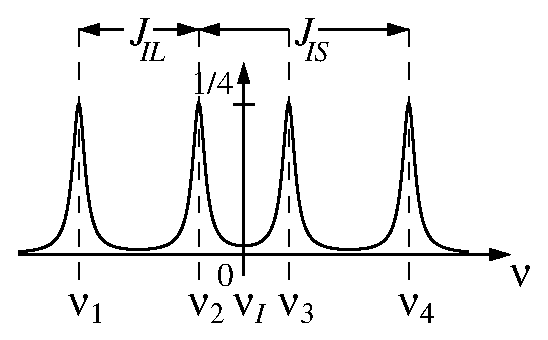
\epsfig{file=ix-isl.eps,width=1.5in}
\end{center}
\caption[Doublet de doublet produit par un système $ISL$]{
\label{fig:ix-isl}
Doublet de doublet produit par un système $ISL$}
\end{figure}

Si les constantes de couplage $J_{IS}$ et $J_{IL}$ sont égales,
on observe trois raies d'intensités 
relatives 1 : 2 : 1 qui constituent un triplet.

L'approximation des faibles couplages permet aussi de traiter les 
problèmes où deux noyaux sont magnétiquement équivalents, sous réserve de 
considérer comme nulle leur constante de couplage.

\section{Cohérences}

Le concept de "cohérence" est utilisé pour faciliter l'écriture des programmes
de phase associés aux séquences d'impulsions ou la mise en place
d'impulsions de gradient de champ statique $\bzerovec$.
Dans les deux cas il s'agit d'enregistrer la partie pertinente du signal
et d'éliminer celle que ne l'est pas.
Au paragraphe \ref{sec:progphaseft} nous avons vu que des imperfections
possibles de l'électronique de réception sont susceptibles
d'introduire des pics indésirables, pics
qui ont été éliminés en faisant varier simultanément les phases
d'émission (des impulsions) et de réception (du signal).
Ce besoin de tri sélectif du contenu du signal
est omniprésent dans les expériences de RMN multi--impulsionnelle.

Les cohérences sont définies de manière très naturelle à
partir de la définition de la matrice densité,
elles sont en fait liées à la manière dont on choisit une base
de matrices densité élémentaires pour décomposer la
matrice densité d'un système.
Cela va d'abord être illustré pour un système à un spin
et sera ensuite généralisé.

La base \{$E/2$, $I_x$, $I_y$, $I_z$\} peut être remplacée par la
base \{$E/2$, $I_+$, $I_-$, $I_z$\} où les matrices $I_+$ et $I_-$, sont 
définies par les relations :
\begin{equation}
I_+ = I_x + i \cdot I_y \qetq I_- = I_x - i \cdot I_y
\end{equation}
ou
\begin{equation}
I_x = \frac{I_+ + I_-}{2} \qetq I_y = \frac{I_+ - I_-}{2i}
\end{equation}

Les opérateurs $I_+$ et $I_-$ sont les cohérences du système à un spin.
Il est possible de voir ce que cela signifie en regardant
l'évolution de $\sigma_1 = I_x = (I_+ + I_-)/2$ 
sous l'action de l'opérateur d'évolution libre
$\phi \cdot I_z$ où $\phi = \omsi t$.
Ceci peut se faire en évaluant d'abord comment évoluent $I_+$ et $I_-$.
En ce qui concerne $I_+ = I_x + i \cdot I_y$ :
\begin{eqnarray}
I_+ & \flham{\phi \cdot I_z} & 
(\cos\phi \cdot I_x + \sin\phi \cdot I_y) + i(\cos\phi \cdot I_y - \sin\phi \cdot I_x) \\
& & = \cos\phi(I_x + i \cdot I_y) -i\sin\phi(I_x + i \cdot I_y) \\
\label{eqn:evoliplus} & & = \exp(-i \phi) \cdot I_+
\end{eqnarray}

De même,
\begin{equation}
\label{eqn:evolimoins}
I_- \flham{\phi \cdot I_z} \exp(+i \phi) \cdot I_-
\end{equation}

L'introduction de $\phi = \omsi t$ n'est pas seulement destinée
à alléger la présentation des calculs.
Elle introduit une unification formelle entre les rotations
de l'aimantation autour des axes transversaux du référentiel tournant
lors des impulsions de radio-fréquence et la rotation autour de l'axe $OZ$ pendant
les périodes de précession.

De manière générale \emph{une cohérence est une matrice densité qui est transformée
en un multiple d'elle même par action du superopérateur lié à
l'évolution libre du système}.
Un mathématicien dirait que les cohérences sont les matrices propres
du super--opérateur hamiltonien.

Pour en revenir à l'évolution de $I_x$, en remplaçant $\phi$ par sa valeur 
on obtient :
\begin{equation}
\label{eqn:evolcoher}
\sigma(t) = \exp(+i \omsi t)/2 \cdot I_- + \exp(-i \omsi t)/2 \cdot I_+
\end{equation}

Le signal observé est en fait le double du coefficient multiplicatif 
associé à la matrice de base $I_-$. 
Si le signal complexe $s(t)$ avait été calculé à partir de l'expression 
$M_x - i.M_y$, $s(t)$ aurait été le coefficient multiplicatif de $I_+$
(à un facteur 2 près).

La matrice densité $\sigma_1$ obtenue immédiatement après l'impulsion de radio-fréquence
traduit l'existence d'une aimantation transversale,
aimantation qui peut être convertie soit en signal évoluant à la pulsation $\omsi$, 
soit à la pulsation $-\omsi$.
Ceci est à rapprocher du fait que $\sigma_1 = I_+/2 + I_-/2$,
que $I_+$ évolue en $\exp(-i \omsi t) \cdot I_+$ et 
que $I_-$ évolue en $\exp(+i \omsi t) \cdot I_-$.
 
On associe aux matrices $I_-$ et $I_+$ une grandeur appelée ordre de 
cohérence (noté $p$) et qui vaut respectivement -1 et +1. 
L'ordre de cohérence $p$ d'une matrice traduit la manière 
dont elle évolue lors d'une rotation autour de $OZ$ : 
une matrice $B_p$ d'ordre bien défini $p$, comme $I_+$ et $I_-$, 
par opposition à $I_x$ et $I_y$ qui en sont des combinaisons,
évolue sous l'action d'un opérateur $\phi . I_z$ selon
\begin{equation}
B_p \flham{\phi \cdot I_z} \exp(-i p \phi) \cdot B_p
\end{equation}

La matrice $I_z$ reste invariante sous l'action des opérateurs d'évolution libre. 
Bien qu'elle ne soit pas associée à la mesure de l'aimantation transversale, on lui attribue 
formellement l'ordre 0 : $\exp(-i 0 \phi) = 1$, indépendamment de $\phi$.
La matrice identité $E$ se voit aussi attribuer un ordre de cohérence nul
du fait de son invariance par toute transformation linéaire.
Ces points seront détaillés ultérieurement, au paragraphe \ref{sec:population}.

L'ordre de cohérence $p$ d'une matrice est aussi couramment désigné sous le
terme "nombre de quanta" de l'état correspondant : 
$I_-$, $I_z$ et $I_+$ sont respectivement des états à -1, 0 (par extension) et +1 quanta.
Le fait que l'aimantation soit mesurée comme le facteur multiplicatif de $I_-$
fait dire que ce sont les états "à -1 quanta" qui sont observables.
Dans un système à un spin nous venons de voir que l'ordre
de cohérence d'un état d'ordre défini est invariante pendant une période
d'évolution libre.
Ce résultat est tout-à-fait général, tant que les phénomènes de relaxation
sont négligés.
Il est clair qu'au bout d'un temps infini l'état de tout système retourne vers
l'ordre 0.
Les impulsions de radio-fréquence sont le moyen par lequel le spectroscopiste
induit des changements d'ordre de cohérence du système et permet, entre autres,
la production d'aimantation transversale mesurable au cours de son retour à
l'équilibre.

\section{Ordre de cohérence et programme de phase}
\label{sec:progphasedensite}
Ce paragraphe fait appel aux notions introduites en \ref{sec:progphaseft}.

On y considère d'abord une impulsion d'angle $\pi/2$ et de phase 
nulle qui transforme $I_z$ ($p=0$) en $-I_y = -(I_+ - I_-)/2i$. 
Lors d'une seconde expérience, on augmente de $\pi/2$ la phase de 
l'impulsion pour former une impulsion $\pi/2_y$.
Cela peut se concevoir comme résultant de l'action successive
d'une impulsion $\pi/2_x$ exercée sur l'aimantation d'équilibre
suivie d'une rotation de $\pi/2$ autour de l'axe $OZ$,
et se justifie aisément en disant que l'axe de rotation $OX$ (première impulsion)
se transforme en $OY$ (seconde impulsion) par rotation de $\pi/2$
autour de $OZ$.
La première étape (l'impulsion $\pi/2_x$) conduit $I_z$ vers $-I_y = -(I_+ - I_-)/2i$.
La seconde étape (la rotation de $\pi/2$ autour de $OZ$)
transforme $I_+$ en $\exp(-i\pi/2) I_+ = -iI_+$
et $I_-$ en $\exp(+i\pi/2) I_- = iI_-$.
Globalement $I_z$ devient $-(-iI_+ - iI-)/2i$ soit $I_x$.

Ce raisonnement peut paraître superflu car le lecteur a remarqué depuis
un certain temps déjà qu'une impulsion $\pi/2_y$ transforme $I_z$ en $I_x$.
Son intérêt consiste à considérer dans son ensemble
les évènements de la séquence impulsion--détection.
L'état du système à la fin de la première impulsion est $-I_y = -(I_+ - I_-)/2i$,
ce qui conduit à $s(t=0)=-i$,
$-i$ étant le double du facteur multiplicatif de $I_-$ à la fin de l'impulsion.
Sachant que $I_-$ évolue en $\exp(-i(-1)\omsi t)I_- = \exp(i\Omega t)I_-$ 
après $t$ secondes,
le signal détecté après l'impulsion de phase nulle est $-i\exp(i\Omega t)$.
Si la phase de l'impulsion est maintenant augmentée de $\pi/2$, $I_-$ est remplacé
par $\exp(+i\pi/2) I_-$ au temps $t=0$ de la détection.
Le signal enregistré est donc simplement multiplié par $\exp(+i\pi/2) = i$,
comme déjà observé en \ref{sec:progphaseft}.
Il suffit de multiplier dans le récepteur le signal par $-i$ pour additionner
de manière constructive les signaux issus des deux impulsions.
Cette multiplication correspond, comme cela a déjà été dit, à une augmentation
$\Delta\phi_R = \pi/2$ de la phase du récepteur.

En retraçant l'origine du résultat, $\Delta\phi_R = \Delta\phi$,
que nous venons d'établir à nouveau, mais par des
moyens qui se prêtent aisément à une généralisation, il apparaît
que l'augmentation de la phase du récepteur doit être égale à la celle
de l'impulsion pour les raisons suivantes :
\begin{itemize}
\item L'aimantation initiale se comporte comme un état à 0 quanta
\item L'impulsion produit un état à -1 quanta
\item Cet état à -1 quanta initial restera à -1 quanta pendant la détection
\item Seul l'état à -1 quanta est détectable
\item L'impulsion produit aussi un état à +1 quanta
\item Cet état à +1 quanta reste à +1 quanta et n'est pas détectable
\item Une augmentation de la phase de l'impulsion de $\Delta\phi$ multiplie $s(t=0)$
par $\exp(-i p \Delta\phi) = \exp(i \Delta\phi)$ car $p(I_-)=-1$
\item $s(t)$ se déduit de $s(0)$ de manière indépendante de la nature de l'impulsion.
\item L'augmentation de la phase du récepteur de $\Delta\phi$ compense exactement
le facteur multiplicatif introduit par l'augmentation de la phase de l'impulsion.
\end{itemize} 

Le raisonnement tenu ici n'est valable que parce que l'aimantation initiale est
décrite par un état à 0 quanta et que l'état détecté est à -1 quanta.
Lorsque ce n'est pas le cas, un résultat analogue mais général peut être obtenu,
résultat qui lie phase du récepteur et phase de la ou des impulsions
de la séquence utilisée.
La démonstration en sera abordée lorsque les cohérences des systèmes
à plusieurs spins auront été définies.

Pour en finir avec ce paragraphe quelque peu théorique,
il est intéressant de voir quelle interprétation donner aux
pics axiaux et fantômes de quadrature dans le cadre du formalisme des cohérences.

Les pics axiaux apparaissent à l'identique quelle que soit
la phase de l'impulsion utilisée.
On peut donc dire que tout se passe comme si le détecteur enregistre
un signal constant, issu d'une cohérence à 0 quanta, associé à une pulsation nulle.

Rappelons que si les amplificateurs des signaux $s_x(t)$ et $s_y(t)$
ont des gains relatifs $1+\delta$ et $1-\delta$ le signal
observé est $s'(t)=\exp(i\omsi t) + \delta\exp(-i\omsi t)$,
ce qui correspond pour le premier terme à la détection normale des -1 quanta
et pour le second terme à la détection des +1 quanta.
Pour se convaincre de cette dernière affirmation, il suffit de se rappeler
que $\exp(-i\Omega t)$ est le facteur multiplicatif de $I_+$ lors de l'évolution
libre de l'aimantation transversale (équation \ref{eqn:evolcoher}).
Les signaux issus de la détection des +1 quanta sont multipliés
par $\exp(-i\pi/2) = -i$ lorsque la phase de l'impulsion est augmentée de $\pi/2$.
L'augmentation de $\pi/2$ de la phase du récepteur multiplie à son tour
le signal par $\exp(-i\pi/2) = -i$.
La contribution provenant de la détection des +1 quanta est donc multipliée
par $(-i)(-i)=-1$, et disparaît par addition des signaux.

Le programme de phase, en additionnant de manière constructive
que les signaux issus de la détection des -1 quanta, élimine
les signaux indésirables aux pulsations 0 et $-\omsi$.

\section{Évolution libre des matrices de base}

Le but de ce paragraphe est de préciser comment évoluent les 
matrices de base des systèmes à un ou plusieurs spins, afin de pouvoir prévoir rapidement 
quelle matrice de base, écrite au temps $t=0$ de l'acquisition du signal
sera responsable de quel groupe de raies dans le spectre.
Il constitue une extension de l'exemple du paragraphe \ref{sec:isl}
et permet d'introduire le concept de cohérence pour les systèmes à
plusieurs spins.

\subsection{Système à un spin, encore}
Dans un système à un spin, $\sigma(t=0) = I_x$ évolue pour donner le signal 
$s(t) = \exp(i \omsi t)$, 
dont la transformée de Fourier $S(\Omega) = A(\omsi) + iD(\omsi)$ a pour
partie réelle la courbe lorentzienne en 
absorption $A(\omsi)$ (figure \ref{fig:absorp}), 
si on tient compte du facteur de relaxation transversale. 
Dans les mêmes conditions, $I_y$ évolue pour donner un signal $s(t) = i\exp(i \omsi t)$
dont la transformée de Fourier $S(\Omega) = -D(\omsi) + iA(\omsi)$
a pour partie réelle la courbe de Lorentz en dispersion $-D(\omsi)$
(figure \ref{fig:dispers}).

\subsection{Système à deux spins}

\subsubsection{Etats non couplés}
L'évolution de $\sigma(t=0) = I_x$ pour un système à deux spins $IS$ 
faiblement couplés fournit le signal 
$2s(t) = \exp(i (\omsi + \pi J) t) + \exp(i (\omsi - \pi J) t)$. 
La partie réelle spectre 
\begin{equation}
S(\Omega) = A(\omsi + \pi J) + iD(\omsi + \pi J) + A(\omsi - \pi J) + iD(\omsi - \pi J)
\end{equation}
présente deux raies 
d'absorption aux pulsations $\omsi + \pi J$ et $\omsi - \pi J$.
Elles constituent un doublet en absorption et en phase.
Ce dernier terme indique que les deux parties du doublet sont de même signe.
Le spectre qui résulte de l'évolution de $I_y$, dans le mêmes conditions,
présente deux raies en dispersion et en phase. 
Les évolutions de $S_x$ et de $S_y$ sont semblables à celles de $I_x$ et $I_y$,
en remplaçant $\omsi$ par $\omss$.
Pour une raison qui apparaîtra au paragraphe suivant, les états
$I_x$, $I_y$, $S_x$ et $S_y$ sont dits "états non couplés" du système $IS$.

Reprenons la question de l'évolution libre de $\sigma(t=0) = I_x$ mais
avec une description utilisant les cohérences.
On peut à ce stade tenter d'écrire $I_+ = I_x + iI_y$ et $I_- = I_x - iIy$
en se rappelant qu'il s'agit de matrices à 16 éléments (4 fois 4) et non plus
de matrices à 4 éléments (2 fois 2) comme pour les systèmes à un spin.

$I_+$ est une matrice d'ordre de cohérence $+1$ 
si une rotation d'angle $\phi$ autour de $OZ$
donne $\exp(-i\phi)I_+$.
Une rotation autour de $OZ$ et d'angle $\phi$ correspond dans ce contexte
au superopérateur associé à l'opérateur $\phi F_z$ où 
\begin{equation}
\label{eqn:operateurf}
F_z = I_z + S_z
\end{equation}
et autrement dit, à l'opérateur $\phi I_z + \phi S_z$.
Etant donné que $\{S_z, I_{\pm}\} = 0$, 
les matrices $I_+$ et $I_-$ sont transformées
en $\exp(-i \phi) I_+$ et $\exp(i \phi) I_-$ par action de $\phi F_z$,
ce qui leur confère respectivement un ordre de cohérence $+1$ et $-1$.

\subsubsection{États couplés}
Il est possible d'écrire $2I_xS_z = (I_+ + I_-)Sz = I_+S_z + I_-S_z$
et facile à vérifier que $I_+S_z$ et $I_-S_z$ sont aussi des matrices respectivement
d'ordre de cohérence +1 et -1 puisque $\{S_z, 2I_{x,y}S_z\} = 0$ et 
$\{I_z, 2I_{x,y}S_z\} = 2\{Iz, I_{x,y}\}S_z$.

L'évolution de $2I_xS_z$ sous l'action de l'opérateur d'évolution libre
$H = \omsi t I_z + \omss t S_z + \pi J t 2I_zS_z$ est décrite par la figure
\ref{fig:evolixsz}.

\begin{figure}[hbt]
\begin{center}
\setlength{\unitlength}{0.9mm}
\begin{picture}(80,50)
 
 \put(0,5){\makebox(0,0)[t]{$2I_xS_z$}}
 \put(20,5){\makebox(0,0)[t]{$2I_yS_z$}}
 \put(40,5){\makebox(0,0)[t]{$\boldsymbol{I_y}$}}
 \put(60,5){\makebox(0,0)[t]{$\boldsymbol{-I_x}$}}
  \put(80,10){\makebox(0,0)[rb]{$\omsi t \cdot I_z$}}
 \put(10,16){\vector(-1,-1){10}}
 \put(10,16){\vector(1,-1){10}}
 \thicklines
 \put(50,16){\vector(-1,-1){10}}
 \put(50,16){\vector(1,-1){10}}
 \thinlines

 \put(10,20){\makebox(0,0)[t]{$2I_xS_z$}}
 \put(50,20){\makebox(0,0)[t]{$\boldsymbol{I_y}$}}
  \put(80,25){\makebox(0,0)[rb]{$\pi J_{IL} t \cdot 2I_zS_z$}}
 \put(30,31){\vector(-2,-1){20}}
 \thicklines
 \put(30,31){\vector(2,-1){20}}
 \thinlines

 \put(30,35){\makebox(0,0)[t]{$\boldsymbol{2I_xS_z}$}}
  \put(80,40){\makebox(0,0)[rb]{$\omss t \cdot 2S_z$}}
 \thicklines
 \put(29.8,46){\vector(0,-1){10}} \put(30.2,46){\vector(0,-1){10}}
 \thinlines

 \put(30,50){\makebox(0,0)[t]{$\boldsymbol{2I_xS_z}$}}

\end{picture}
 \caption[Évolution de $2I_xS_z$, système $IS$]{\label{fig:evolixsz} 
 Évolution libre d'un état $2I_xS_z$ d'un système $IS$.}
\end{center}
\end{figure}

Contrairement à ce qui se passe pour l'évolution de $I_x$ où, à la fin du calcul, 
le coefficient multiplicatif de $I_x$ et $I_y$ varie en $\cos(\pi J t)$, 
ici ces coefficient varient en $\sin(\pi J t)$. 
Ainsi 
\begin{eqnarray}
s(t) & = & -\sin(\omsi t)\sin(\pi J t) + i\cos(\omsi t)\sin(\pi J t) \\
& = & i\exp(i\omsi t)\sin(\pi J t)
\end{eqnarray}
Le développement de la fonction sinus en exponentielles complexes :
\begin{equation}
s(t) = \exp(i (\omsi t + \pi J)t)/2 - \exp(i (\omsi t - \pi J)t)/2
\end{equation}
fait apparaître deux raies en absorption mais de signes opposés :
on parle alors d'un doublet antiphase. 
Il en est de même pour $2I_zS_x$, $2I_yS_z$ et $2I_zS_y$
Ces matrices de base décrivent des états du système appelés "états couplés".

La figure \ref{fig:ixysz-is} montre les doublets produits par un noyau
$I$ couplé faiblement à partir des états (a) $2I_xS_z$ et (b) $2I_yS_z$.

\begin{figure}[hbt]
\begin{center}
$a$\hspace{1.5in}\hspace{1cm}$b$\hspace{1.5in}$\mbox{ }$\\
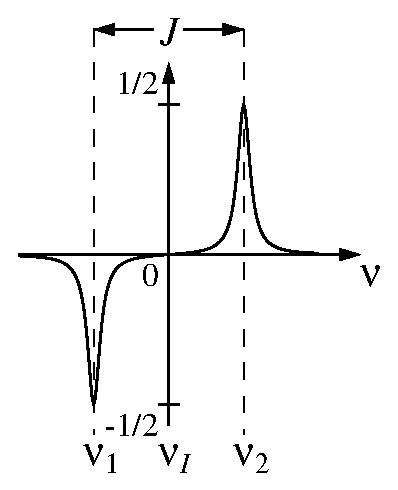
\epsfig{file=ixsz-is.eps,width=1.5in} \hspace{1cm}
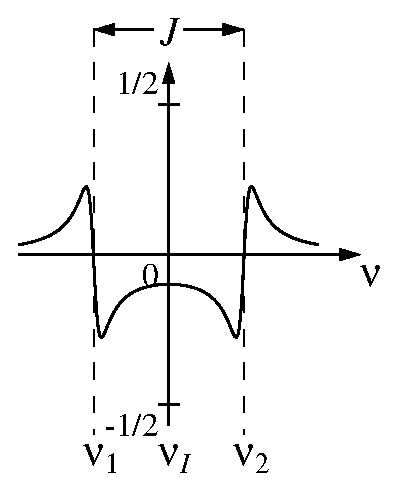
\epsfig{file=iysz-is.eps,width=1.5in}
\end{center}
\caption[Doublets antiphases produits par un système $IS$]{
\label{fig:ixysz-is}
(a) doublet antiphase en absorption issu de $I_xS_z$,
(b) doublet antiphase en dispersion issu de $I_yS_z$}
\end{figure}

Les états $I_-$ et $I_-S_z$ sont, nous l'avons vu, des matrices
d'ordre de cohérence -1.
Ils se convertissent l'un en l'autre par action de l'opérateur
d'évolution libre mais conservent donc l'ordre de cohérence -1 :
\begin{eqnarray}
I_x & \flham{\pi J t \cdot 2I_zSz} &
\cos(\pi J t) \cdot I_x + \sin(\pi J t) \cdot 2I_yS_z \\ 
I_y & \flham{\pi J t \cdot 2I_zSz} &
\cos(\pi J t) \cdot I_y - \sin(\pi J t) \cdot 2I_yS_z
\end{eqnarray}
D'où
\begin{eqnarray}
I_{\pm} = I_x \pm iI_y & \flham{\pi J t \cdot 2I_zSz} &
\cos(\pi J t) \cdot I_{\pm} \mp i \sin(\pi J t) \cdot 2I_{\pm}S_z \\
\label{eqn:evolipm-is} I_{\pm} & \flham{Ht} &
\exp(\mp i \omsi t)(\cos(\pi J t) \cdot I_{\pm} \mp i \sin(\pi J t) \cdot 2I_{\pm}S_z)
\end{eqnarray}
De manière identique :
\begin{equation}
\label{eqn:evolipmsz-is} 2I_{\pm}S_z \flham{Ht}
\exp(\mp i \omsi t)(\cos(\pi J t) \cdot 2I_{\pm}S_z \mp i \sin(\pi J t) \cdot I_{\pm})
\end{equation}

Les matrices $I_{\pm}$ et $2I_{\pm}S_z$ ne sont pas des cohérences du 
système étudié, toutefois leur ordre de cohérence n'est pas modifié
par l'évolution libre, puisqu'elles évoluent comme une somme de
deux matrices de même ordre de cohérence.

Ce résultat est très général : \emph{l'évolution libre de fait pas varier
l'ordre de cohérence d'un état}.

A partir de la demi somme et de la demi différence des équations 
\ref{eqn:evolipm-is} et \ref{eqn:evolipmsz-is},
du fait que $I_{\pm}$ est en fait $I_{\pm}E_S$,
et des définitions :
\begin{eqnarray}
S_{\al} & = & \frac{E_S + 2S_z}{2} \\
S_{\be} & = & \frac{E_S - 2S_z}{2}
\end{eqnarray}
on obtient
\begin{eqnarray}
\label{eqn:evolipmsa-is} I_{\pm}S_{\al} & \flham{Ht} &
\exp(\mp i (\omsi + \pi J)t) \cdot I_{\pm}S_{\al} \\
\label{eqn:evolipmsb-is} I_{\pm}S_{\be} & \flham{Ht} &
\exp(\mp i (\omsi - \pi J)t) \cdot I_{\pm}S_{\be}
\end{eqnarray}
ce qui prouve que les matrices $I_{\pm}S_{\al}$ et $I_{\pm}S_{\be}$ 
sont des cohérences du système $IS$ faiblement couplés,
d'ordre de cohérence $\pm 1$.
Il en est de même, par symétrie, pour les matrices $I_{\al}S_{\pm}$ et $I_{\be}S_{\pm}$.

Les fréquences d'évolution de ces cohérences à simple quanta sont exactement les
fréquences des transitions observables dans le diagramme énergétique du système $IS$.
L'ordre de cohérence d'un terme de la matrice densité
correspond de fait à la valeur de $\Delta m_s$ de la transition qui lui est associée.
Ce point est à la base du lien qui sera fait entre le formalisme
de la matrice densité et la généralisation du modèle de Bloch.

\subsubsection{États à 0 et double quanta}
Parmi les états dont il n'a pas encore été question figurent ceux décrits
par les opérateurs $2I_{x,y}S_{x,y}$.
Le fait est qu'ils sont impossibles à produire à partir de l'état d'équilibre
en utilisant une seule impulsion idéale, ce qui
explique qu'ils n'aient pas encore été rencontrés avant ce point du texte.
Ils sont cependant impliqués dans certaines expériences multi--impulsionnelles
de grande importance pratique.
La matrice $2I_xS_x$ s'exprime en fonction de $I_+$, $I_-$, $S_+$, $S_-$
par la relation $2I_xS_x = (I_+ + I_-)(S_+ + S_-)/2$ soit 
$I_+S_+/2 + I_+S_-/2 + I_-S_+/2 + I_-S_-/2$. 

A nouveau l'action de l'opérateur $\phi \cdot F_z$ sur ces quatre derniers
opérateurs montre que ce sont des cohérences d'ordre respectivement +2, 0, 0 et -2.
On parle alors de cohérence à double et à zero quanta.
Il est donc certain que l'évolution libre de $2I_xS_x$ ne fera apparaître 
aucune aimantation mesurable.
La matrice $2I_xS_x$ évolue néanmoins, mais sans faire apparaître la constante de 
couplage puisque $2I_zS_z$ et $2I_xS_x$ commutent, comme
indiqué sur la figure \ref{fig:evolixsx}.

\begin{figure}[hbt]
\begin{center}
\setlength{\unitlength}{0.9mm}
\begin{picture}(80,50)
 
 \put(0,5){\makebox(0,0)[t]{$2I_xS_x$}}
 \put(20,5){\makebox(0,0)[t]{$2I_xS_y$}}
 \put(40,5){\makebox(0,0)[t]{$2I_yS_x$}}
 \put(60,5){\makebox(0,0)[t]{$2I_yS_y$}}
  \put(80,10){\makebox(0,0)[rb]{$\omss t \cdot S_z$}}
 \put(10,16){\vector(-1,-1){10}}
 \put(10,16){\vector(1,-1){10}}
 \put(50,16){\vector(-1,-1){10}}
 \put(50,16){\vector(1,-1){10}}

 \put(10,20){\makebox(0,0)[t]{$2I_xS_x$}}
 \put(50,20){\makebox(0,0)[t]{$2I_yS_x$}}
  \put(80,25){\makebox(0,0)[rb]{$\omsi t \cdot I_z$}}
 \put(30,31){\vector(-2,-1){20}}
 \put(30,31){\vector(2,-1){20}}

 \put(30,35){\makebox(0,0)[t]{$2I_xS_x$}}
  \put(80,40){\makebox(0,0)[rb]{$\pi J t \cdot 2I_zS_z$}}
 \put(29.8,46){\vector(0,-1){10}} \put(30.2,46){\vector(0,-1){10}}

 \put(30,50){\makebox(0,0)[t]{$2I_xS_x$}}

\end{picture}
 \caption[Evolution de $2I_xS_x$, système $IS$]{\label{fig:evolixsx} 
 Evolution libre d'un état $2I_xS_x$ d'un système $IS$.}
\end{center}
\end{figure}

Dans $\sigma(t)$, le coefficient multiplicatif de $2I_xS_x$ est 
$\cos(\omsi t) \cos(\omss t)$, qui vaut aussi 
$\cos((\omsi + \omss)t)/2 + \cos((\omsi - \omss)t)/2$. 
Les pulsations $\omsi + \omss$ et $\omsi - \omss$ sont les 
pulsations associées aux transitions à $\pm 2$ et 0 quanta du système $IS$. 
Un calcul identique montre que chacune des quatre matrices associées aux transitions à  
0 et $\pm 2$ quanta évolue pour donner des combinaisons de ces quatre matrices.
Cette observation est compatible avec la décomposition des matrices 
$2I_{x,y}S_{x,y}$ en termes d'ordre de cohérence 0 et $\pm 2$.
En effet, on peut écrire :
\begin{eqnarray}
& & I_{\pm}S_{\pm} \flham{\pi J t \cdot 2I_zS_z} I_{\pm}S_{\pm} \nonumber\\
& & \quad \flham{\omsi t I_z} 
\exp(i\mp\omsi t)I_{\pm}S_{\pm} \nonumber\\
& & \quad \flham{\omss t S_z}
\exp(i\mp\omsi t) \exp(i\mp\omss t) I_{\pm}S_{\pm} \nonumber\\
& & \quad\quad = \exp(i(\mp\omsi \mp\omss)t) I_{\pm}S_{\pm} 
\end{eqnarray}

Il apparaît donc ici que les matrices $I_{\pm}S_{\pm}$ sont des cohérences.
Leur fréquence d'évolution est égale aux fréquences des transitions
à zéro et double quanta déduites du diagramme énergétique du système $IS$.

\subsubsection{Ordres de cohérence partiels}
On constate que l'ordre de cohérence d'un état s'obtient par addition des ordres
de cohérence individuels associés aux noyaux $I$ et $S$ considérés séparément.
En fait, considérons une cohérence générale $I_{\lambda}S_{\mu}$, avec $\lambda$, $\mu$
valant $z$, $+$, $-$, ou 0 pour signifier que l'opérateur n'y figure pas
(et donc d'ordre de cohérence nul !).
Alors,
\begin{eqnarray}
& &I_{\lambda}S_{\mu} \flham{\phi \cdot Iz}
\exp(-i p(I_{\lambda}) \phi) \cdot I_{\lambda}S_{\mu}\\
& &I_{\lambda}S_{\mu} \flham{\phi \cdot Sz}
\exp(-i p(S_{\mu}) \phi) \cdot I_{\lambda}S_{\mu}\\
& &I_{\lambda}S_{\mu} \flham{\phi \cdot Fz}
\exp(-i p(I_{\lambda} \phi)\exp(-i p(S_{\mu}) \phi) \cdot I_{\lambda}S_{\mu}\nonumber\\
& & \quad = \exp(-i (p(I_{\lambda})+p(S_{\mu})) \phi) \cdot I_{\lambda}S_{\mu}
\end{eqnarray}
ce qui montre bien que
\begin{equation}
p(I_{\lambda}S_{\mu}) = p(I_{\alpha}) + p(S_{\mu})
\end{equation}

Les quantités $p(I_{\lambda})$ et $p(S_{\mu})$ sont appelées ordres de cohérence partiels,
quantités dont la somme est l'ordre de cohérence total.
Il est important aussi de noter que, dans la mesure où on ne considère
que des systèmes de spins faiblement couplés,
\emph{les ordres de cohérence partiels sont invariants au cours des périodes
d'évolution libre}. 

\subsubsection{Populations}
Les matrices $E$, $I_z$, $S_z$, $2I_zS_z$ sont invariantes par action des opérateurs 
d'évolution libre et ne sont sujettes qu'aux phénomènes liés à la relaxation longitudinale.
Ces matrices ne constituent pas des cohérences mais des populations (voir \ref{sec:population}),
bien que leur invariance sous l'action de $\phi \cdot F_z$ permettent de leur
attribuer un ordre de cohérence global nul, somme d'ordres de cohérence partiels nuls.

Il faut bien noter qu'un état comme $I_+S_-$, bien que d'ordre de cohérence nul,
n'est pas une population, car il n'est pas invariant par action de $\phi \cdot F_z$.

\subsection{Système à trois spins}
Les matrices de base utilisées pour décrire les systèmes à trois spins sont classables en 
sept catégories suivant les ordres de cohérences qui leur sont associés et l'existence 
d'états couplés.
Pour chaque catégorie nous donnerons dans la table \ref{tab:isl}
un exemple représentatif et la 
possibilité ou non de donner de l'aimantation observable
par évolution libre.

\begin{table}[hbt]
\begin{center}
\begin{tabular}{llcc}
 & Catégorie & Exemple & Détectable\\[0.5ex] 
1 & Population (pseudo-ordre 0) & $4I_zS_zL_z$ & non \\
2 & Ordre $\pm 1$ non couplé & $L_x$ & oui \\
3 & Ordre $\pm 1$ couplé 1 fois & $2S_zL_x$ & oui \\
4 & Ordre $\pm 1$ couplé 2 fois & $4I_xL_zS_z$ & oui \\
5 & Ordre 0, $\pm 2$ non couplé & $2S_xL_y$ & non \\
6 & Ordre 0, $\pm 2$ couplé & $4I_xS_yL_z$ & non \\
7 & Ordre $\pm 1$, $\pm 3$ & $4I_xS_xL_x$ & non
\end{tabular}
\caption{\label{tab:isl}Classification des opérateurs pour les systèmes à trois spins}
\end{center}
\end{table}

Les catégories originales introduites à cause de la présence d'un troisième noyau sont 
numérotées 4, 6 et 7.

Il convient d'insister ici sur le fait que l'état $2S_zL_x$,
ligne 3 du tableau \ref{tab:isl},
n'est pas détectable en tant que tel, mais que son évolution libre conduit
à un état observable.
Il en est de même pour les états correspondants à la ligne 4.

Considérons l'évolution des matrices $I_x$ (type 2), $2I_xS_z$ (type 3)
et $4I_xS_zL_z$ (type 4) selon l'opérateur 
d'évolution libre associé aux systèmes de trois noyaux faiblement couplés. 
Ces trois matrices commutent avec les opérateurs 
$\omss t \cdot S_z$, $\omsl t \cdot L_z$ et $\pi J_{SL} t \cdot 2S_zL_z$.
De plus, on ne s'intéresse qu'à la nature des résonances du noyau $I$ couplé à S et L, 
qui doit être indépendante de l'offset de $I$, ce qui permet de choisir $\omsi = 0$. 
Ceci revient à ne pas prendre en compte l'opérateur $\omsi t \cdot I_z$
Parmi les 6 termes initiaux de l'opérateur d'évolution libre,
seuls $\pi J_{IS} t \cdot 2I_zS_z$ et $\pi J_{IL} t \cdot 2I_zL_z$ restent à considérer.

Le calcul de l'évolution de $I_x$ a déjà été présenté en \ref{sec:isl}
et conduit à quatre raies en absorption de même signe (on dit aussi "en phase").

L'évolution de $2I_xS_z$ s'écrit :

\begin{figure}[hbt]
\begin{center}
\setlength{\unitlength}{0.9mm}
\begin{picture}(90,35)
 
 \put(0,5){\makebox(0,0)[t]{$2I_xS_z$}}
 \put(20,5){\makebox(0,0)[t]{$4I_yS_zL_z$}}
 \put(40,5){\makebox(0,0)[t]{$\boldsymbol{I_y}$}}
 \put(60,5){\makebox(0,0)[t]{$-2I_xL_z$}}
  \put(90,10){\makebox(0,0)[rb]{$\pi J_{IL} t \cdot 2I_zL_z$}}
 \put(10,16){\vector(-1,-1){10}}
 \put(10,16){\vector(1,-1){10}}
 \thicklines
 \put(50,16){\vector(-1,-1){10}}
 \thinlines
 \put(50,16){\vector(1,-1){10}}

 \put(10,20){\makebox(0,0)[t]{$2I_xS_z$}}
 \put(50,20){\makebox(0,0)[t]{$\boldsymbol{I_y}$}}
  \put(90,25){\makebox(0,0)[rb]{$\pi J_{IS} t \cdot 2I_zS_z$}}
 \put(30,31){\vector(-2,-1){20}}
 \thicklines
 \put(30,31){\vector(2,-1){20}}
 \thinlines
 
 \put(30,35){\makebox(0,0)[t]{$\boldsymbol{2I_xS_z}$}}

\end{picture}
 \caption[Evolution de $2I_xS_z$, système $ISL$]{\label{fig:evolixszl0} 
 Evolution libre d'un état $2I_xS_z$ d'un système $ISL$.}
\end{center}
\end{figure}

Ainsi
\begin{eqnarray}
s(t) & = & i\sin(\pi J_{IS} t)\cos(\pi J_{IL} t)\\
& = & i \sin(\pi(J_{IS}+J_{IL})t)/2 + i \sin(\pi(J_{IS}-J_{IL})t)/2
\end{eqnarray}

En transformant les fonctions sinus en exponentielles complexes
et après transformation de Fourier,
on obtient quatre raies en absorption de fréquences et d'intensités indiquées ci-dessous :
\begin{eqnarray*}
\mbox{Fréquence} & & \mbox{Intensité} \\[0.5ex]
+J_{IS}+J_{IL} & & +1/4 \\
+J_{IS}-J_{IL} & & +1/4 \\
-J_{IS}+J_{IL} & & -1/4 \\
-J_{IS}-J_{IL} & & -1/4 
\end{eqnarray*}

On retrouve $J_{IS}$ entre deux raies en antiphase et $J_{IL}$ entre deux raies en phase. 
Dans cet exemple $J_{IS}$ est appelé couplage actif car il intervient 
dans l'évolution de $2I_xS_z$ à la fois sur $I_x$ et sur $S_z$.
$J_{IL}$ est ici un couplage inactif (ou passif) : il n'intervient dans l'évolution de 
$2I_xS_z$ que sur $I_x$. 
Un couplage actif donne lieu à une paire de pics antiphase alors 
qu'un couplage inactif donne lieu à une paire de raies en phase.

L'évolution de $I_x$ ne conduit qu'à des pics en phase 
puisque tous les couplages sont passifs.

Dans l'évolution de $4I_xS_zL_z$ les constantes de couplage 
$J_{IL}$ et $J_{IS}$ sont toutes deux actives :

\begin{figure}[hbt]
\begin{center}
\setlength{\unitlength}{0.9mm}
\begin{picture}(90,35)
 
 \put(0,5){\makebox(0,0)[t]{$4I_xS_zL_z$}}
 \put(20,5){\makebox(0,0)[t]{$2I_yL_z$}}
 \put(40,5){\makebox(0,0)[t]{$2I_yS_z$}}
 \put(60,5){\makebox(0,0)[t]{$\boldsymbol{-2I_x}$}}
  \put(90,10){\makebox(0,0)[rb]{$\pi J_{IS} t \cdot 2I_zS_z$}}
 \put(10,16){\vector(-1,-1){10}}
 \put(10,16){\vector(1,-1){10}}
 \put(50,16){\vector(-1,-1){10}}
 \thicklines
 \put(50,16){\vector(1,-1){10}}
 \thinlines

 \put(10,20){\makebox(0,0)[t]{$4I_xS_zL_z$}}
 \put(50,20){\makebox(0,0)[t]{$\boldsymbol{2I_yS_z}$}}
  \put(90,25){\makebox(0,0)[rb]{$\pi J_{IL} t \cdot 2I_zL_z$}}
 \put(30,31){\vector(-2,-1){20}}
 \thicklines
 \put(30,31){\vector(2,-1){20}}
 \thinlines
 
 \put(30,35){\makebox(0,0)[t]{$\boldsymbol{4I_xS_zL_z}$}}

\end{picture}
 \caption[Évolution de $4I_xS_zL_z$, système $ISL$]{\label{fig:evolixszlz} 
 Évolution libre d'un état $4I_xS_zL_z$ d'un système $ISL$.}
\end{center}
\end{figure}

Ainsi,
\begin{eqnarray}
s(t) & = & -\sin(\pi J_{IS} t)\sin(\pi J_{IL} t)\\
& = & \cos(\pi(J_{IS}+J_{IL})t)/2 - \cos(\pi(J_{IS}-J_{IL})t)/2
\end{eqnarray}
En transformant les fonctions cosinus en exponentielles complexes
et après transformation de Fourier,
on obtient quatre raies en absorption de fréquences et d'intensités indiquées ci-dessous :
\begin{eqnarray*}
\mbox{Fréquence} & & \mbox{Intensité} \\[0.5ex]
+J_{IS}+J_{IL} & & +1/4 \\
+J_{IS}-J_{IL} & & -1/4 \\
-J_{IS}+J_{IL} & & -1/4 \\
-J_{IS}-J_{IL} & & +1/4 
\end{eqnarray*}
Les pics distants de $J_{IS}$ d'une part et de $J_{IL}$
d'autre part sont bien en antiphase.

La figure \ref{fig:ixzz-isl} montre les doublets de doublets produits par un noyau
$I$ couplé faiblement aux noyaux $S$ et $L$ à partir des états (a) $2I_xS_z$
et (b) $4I_xS_zL_z$.

\begin{figure}[hbt]
\begin{center}
$a$\hspace{1.5in}\hspace{1cm}$b$\hspace{1.5in}$\mbox{ }$\\
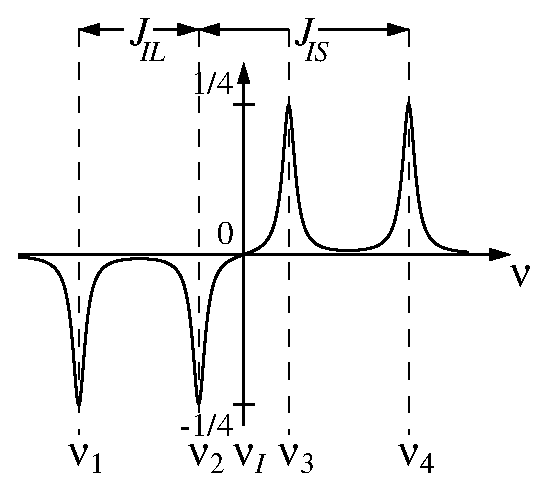
\epsfig{file=ixsz-isl.eps,width=1.5in} \hspace{1cm}
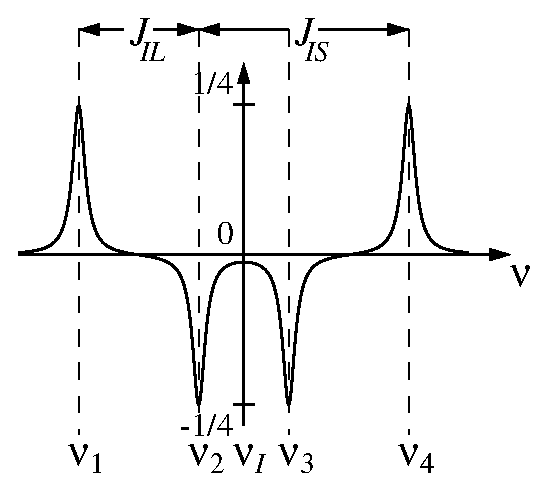
\epsfig{file=ixszlz-isl.eps,width=1.5in}
\end{center}
\caption[Doublets de doublets produits par un système $ISL$]{
\label{fig:ixzz-isl}
(a) Doublet de doublet issu de $2I_xL_z$, antiphase pour $S$ 
(b) doublet de doublet issu de $4I_xS_zL_z$, doublement antiphase (pour $S$ et $L$)}
\end{figure}

Il est intéressant de noter qu'une matrice de base 
comme $4I_xS_xL_x$ ne donne aucune aimantation 
observable alors qu'elle s'exprime aussi comme 
$(I_+ + I_-)(S_+ + S_-)(L_+ + L_-)/2$ et 
contient donc des termes comme $I_+S_-L_-$ d'ordre de cohérence total
égal à $-1$. 
L'existence d'un terme d'ordre de cohérence $-1$ est en effet une condition nécessaire 
mais non suffisante à l'obtention d'un signal.
La production d'un signal détectable reste l'exclusivité des opérateurs
$I_-$, $S_-$ et $L_-$.
